\section{Real time formalism}\label{ss:RTapproach}
We illustrate the real time approach for calculating the reduced density matrix of a subsystem in the Hamiltonian description.
This method is suitable for the numerical computation once we discretize the spacetime to lattice.
We describe only the bosonic case here and defer the fermionic case to the Appendix \ref{ss:RTFermion}.

\subsection{Two coupled harmonic oscillators}
To illustrate the real time approach, we start with a simple example of two coupled harmonic oscillators \cite{Srednicki:1993im,Bombelli:1986rw}; see Fig.\,\ref{fig:HarmChain}.
Suppose this system is described by the Hamiltonian,
\begin{align}\label{TwoHarmH}
H = \frac{1}{2}\left[ p_A^2 + p_B^2 + k(x_A^2 + x_B^2) + l (x_A - x_B)^2 \right] \ ,
\end{align}
where $x_{A,B}$ and $p_{A,B}$ are the positions and the conjugate momenta of the two oscillators, and $k$ and $l$ are related to their mass and the coupling.
First, we want to find the ground state wave function of the system.
To this end, we introduce new variables $x_\pm = (x_A \pm x_B)/\sqrt{2},~ \omega_+ = k^{1/2}$, and $\omega_- = (k + 2l)^{1/2}$.
In these new variables, the Hamiltonian is for two \emph{uncoupled} harmonic oscillators and the Schr{\"o}dinger equation becomes
\begin{align}
	 \frac{1}{2}\left[ - \partial_+^2 - \partial_-^2 + \omega_+^2 x_+^2 + \omega_-^2 x_-^2\right] \Psi (x_+, x_-) = E\, \Psi (x_+, x_-)  \ .
\end{align}
Then the ground state wave function is the product of two copies of the ground state wave function of one harmonic oscillator,
\begin{align}\label{TwoHarmGS}
\Psi  (x_+, x_-) = \frac{(\omega_+ \omega_-)^{1/4}}{\pi^{1/2}} \exp\left[ - \frac{\omega_+ x_+^2 + \omega_- x_-^2}{2}\right] \ ,
\end{align}
with the energy $E = (\omega_+ + \omega_-)/2$.
The overall factor is chosen so that the wave function is normalized to be $\int_{-\infty}^\infty \d x_A \int_{-\infty}^\infty \d x_B |\Psi (x_A, x_B)|^2 = 1$ where we denote the wave function in the original variables $x_A$ and $x_B$ by the same symbol $\Psi (x_A, x_B)$.

Next we trace out the oscillator at $x_B$ and construct the reduced density matrix $\rho_A$ for the oscillator at $x_A$.
If we represent the ground state wave function as $\Psi (x_A, x_B) = (\langle x_A| \otimes \langle x_B|)| \Psi\rangle$,
then the reduced density matrix follows as
\begin{align}\label{rhoATwoHarm}
\begin{aligned}
\rho_A (x_A, x_A') &=  \langle x_A| \tr_B \left(|\Psi\rangle \langle \Psi|\right) | x_A'\rangle \ ,\\
&= \int_{-\infty}^\infty \d x_B \, \Psi(x_A, x_B)\,\Psi^\ast (x_A', x_B) \ , \\
&= \sqrt{\frac{\gamma - \beta}{\pi}}\, \exp\left[ -\frac{\gamma}{2}(x_A^2 + x_A'^2) + \beta\, x_A x_A'\right] \ ,
\end{aligned}
\end{align}
where we introduced the parameters 
\begin{align}
\beta = \frac{(\omega_+ - \omega_-)^2}{4(\omega_+ + \omega_-)} \ , \qquad \gamma = \frac{2\omega_+ \omega_-}{\omega_+ + \omega_-} + \beta \ .
\end{align}

Finally, we need the eigenvalues of the reduced density matrix to compute the entanglement entropy.
The eigenfunction $f_n$ with the eigenvalue $p_n$ must satisfy
\begin{align}
\int_{-\infty}^\infty \d x'\, \rho_A (x, x')\,f_n(x') = p_n\, f_n (x) \ ,
\end{align}
and the solution is given by 
\begin{align}\label{EigenTwoHarm}
\begin{aligned}
f_n (x) &= H_n (\alpha^{1/2} x)\, e^{-\frac{\alpha x^2}{2}} \ ,\qquad (n=0,1,2,\cdots) \ ,
\end{aligned}
\end{align}
where $\alpha = (\omega_+ \omega_-)^{1/2}$ and $H_n$ is the Hermite polynomial.
The eigenvalue $p_n$ is 
\begin{align}\label{Two_harmonic_eigen}
	p_n = (1-\xi)\,\xi^n \ , \qquad \xi = \frac{\beta}{\alpha + \gamma} \ .
\end{align}
One way to derive the eigenfunction is to expand the reduced density matrix by the Hermite polynomial,
\begin{align}
\begin{aligned}
	\rho_A (x, x') &= \sqrt{\frac{\alpha}{\pi}}\,(1-\xi)\,e^{-\frac{\alpha}{2}(x^2 + x'^2)} \\
		&\qquad \cdot \sum_{n=0}^\infty \frac{\xi^n}{2^n n!}  \,H_n(\alpha^{1/2} x) \,H_n(\alpha^{1/2} x') \ ,
\end{aligned}
\end{align}
and use the orthogonality,
\begin{align}
	\int_{-\infty}^\infty \d x\, e^{-x^2} H_n(x)\, H_m(x) = \sqrt{\pi}\,2^n  n!\,\delta_{nm} \ .
\end{align}
Having diagonalized the reduced density matrix, we are ready to obtain the entanglement entropy from the eigenvalue Eq.\,\eqref{Two_harmonic_eigen},
\begin{align}
\begin{aligned}
S_A &=- \sum_{n=0}^\infty\, p_n \log p_n \ , \\
	&= - \log(1-\xi) - \frac{\xi}{1-\xi}\log\xi \ .
\end{aligned}
\end{align}


\subsection{$N$-coupled harmonic oscillators}
It is straightforward to generalize the model Eq.\,\eqref{TwoHarmH} of two harmonic oscillators to a system of $N$-coupled harmonic oscillators (see Fig.\,\ref{fig:HarmChain})
\begin{align}\label{NHarm}
H = \frac{1}{2}\sum_{i=1}^N \pi_i^2 + \frac{1}{2}\sum_{i,j=1}^N \phi_i \,K_{ij}\, \phi_j \ ,
\end{align}
where $K$ is a real symmetric matrix and $\pi_i$ is a canonical conjugate momentum of the oscillator $\phi_i$ satisfying the commutation relation,\footnote{The oscillator and conjugate momentum are considered as Hermitian operators.}
\begin{align}\label{CCR_phi}
	[\phi_i, \pi_j]=\i\,\delta_{ij} \ . 
\end{align}
It reduces to the previous model Eq.\,\eqref{TwoHarmH} for $N=2$, $K_{11}=K_{22} = k+l$ and $K_{12} = -l$.
Instead of repeating the arguments in the literature \cite{Srednicki:1993im,Bombelli:1986rw},
we adopt a different method that suites for numerical computation.

\begin{figure}[htbp]
\centering
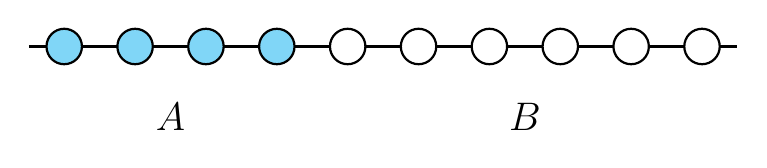
\begin{tikzpicture}[thick, scale=0.45]
	\draw (-1,0) --++(20,0);
	\draw[fill=cyan!50] (0,0) circle (0.5);
	\draw[fill=cyan!50] (2,0) circle (0.5);
	\draw[fill=cyan!50] (4,0) circle (0.5);
	\draw[fill=cyan!50] (6,0) circle (0.5);
	\draw[fill=white] (8,0) circle (0.5);
	\draw[fill=white] (10,0) circle (0.5);
	\draw[fill=white] (12,0) circle (0.5);
	\draw[fill=white] (14,0) circle (0.5);
	\draw[fill=white] (16,0) circle (0.5);
	\draw[fill=white] (18,0) circle (0.5);
	\node at (3,-2) {\Large $A$};
	\node at (13, -2) {\Large $B$};
\end{tikzpicture}
\caption{\label{fig:HarmChain} A system of $N$-coupled harmonic oscillators. Here the total size of the system is $N=10$ and the subsystem $A$ (blue) consists of four oscillators from the left.}
\end{figure}


First, we introduce creation and annihilation operators $a_I$ and $a_I^\dagger$ satisfying the commutation relation $[a_I, a_J^\dagger] = \delta_{IJ}$.
Note that the new indices $I$ and $J$ are different from the indices $i$ and $j$ labeling the lattice site.
They parametrize the Fock space generated by $a_I$ and $a_I^\dagger$.
We assume the operators $a_I$ and $ a_I^\dagger$ are linearly related to the original oscillators $\phi_i$ and $ \pi_j$ with indices $i$ and $j$ in the region $A$ by \cite{Casini:2009sr},
\begin{align}\label{Phi_to_a}
\begin{aligned}
	\phi_i &= \alpha_{iI} (a_{I}^\dagger + a_{I}) \ , \\
	\pi_j &= -\i\, \beta_{jJ} (a_J^\dagger - a_J) \  ,
\end{aligned}
\end{align}
where $\alpha_{iI}$ and $\beta_{jJ}$ are real matrices with the mixed indices of the coordinate space and the Fock space.
These matrices are not independent of each other due to the commutation relation Eq.\,\eqref{CCR_phi} and have to be real matrices satisfying
\begin{align}\label{alphabet}
\alpha\, \beta^T = -\frac{1}{2} \ .
\end{align}
We now {\it assume} that there exists a (modular) Hamiltonian bilinear in the creation and annihilation operators,
\begin{align}
	H_A= \sum_{I} \epsilon_I\, a^\dagger_I a_I \ ,
\end{align}
which generates the reduced density matrix \cite{peschel1999density,chung2000density},
\begin{align}\label{rhoA_ansatz}
\rho_A = \prod_{I\in A} (1 - e^{-\epsilon_I}) \, e^{-H_A} \ .
\end{align}
In order to determine the spectrum $\epsilon_I$, we compare the two-point functions $\langle \phi_i\, \pi_j\rangle = \i\, \delta_{ij}/2$, $X_{ij} \equiv \langle \phi_i \,\phi_j\rangle$ and $P_{ij} = \langle \pi_i \,\pi_j\rangle$ in the subsystem $A$ with those evaluated with the ansatz Eq.\,\eqref{rhoA_ansatz},
\begin{align}\label{XPD}
\begin{aligned}
X_{ij} &= \tr_A (\rho_A\, \phi_i \,\phi_j) \ , \\
P_{ij} &= \tr_A (\rho_A\, \pi_i\, \pi_j) \ , \\
\frac{\i}{2}\delta_{ij}  &= \tr_A (\rho_A\, \phi_i\, \pi_j) \ .
\end{aligned}
\end{align}
The right hand sides can be diagonalized by the coefficient matrices $\alpha$ and $\beta$ in Eq.\,\eqref{Phi_to_a}:
\begin{align}\label{XPDeqs}
\begin{aligned}
X &= \alpha\, (2n+1)\, \alpha^T \ , \\
P &= \beta\, (2n+1)\, \beta^T \ ,
\end{aligned}
\end{align}
where $n$ is the diagonal matrix with entries,
\begin{align}
n_{IJ} = \tr_A (\rho_A\, a_I^\dagger a_J ) = \frac{\delta_{IJ}}{e^{\epsilon_I} - 1} \ .
\end{align}
We can read off the spectrum $\epsilon_I$ of the reduced density matrix from the matrix product $XP$ that is also diagonalized with Eq.\,\eqref{alphabet} as
\begin{align}
XP = \frac{1}{4} \alpha\, (2n+1)^2 \alpha^{-1} \ .
\end{align}
Comparing the eigenvalues of the matrices in both sides, we find
\begin{align}\label{EigenRel1}
\nu_I = \frac{1}{2}\coth \frac{\epsilon_I}{2} \ ,
\end{align}
where $\nu_I$ are the eigenvalues of $C=\sqrt{XP}$.


The entanglement entropy follows from the limit of the R{\'e}nyi entropy Eq.\,\eqref{RenyiEE}.
Since the trace of the $n^{th}$ power of $\rho_A$ is given by
\begin{align}
\begin{aligned}
\tr_A( \rho_A^n) &= \prod_{I}\frac{(1- e^{-\epsilon_I})^n}{1- e^{-n \epsilon_I}} \ ,\\
	&= \prod_{I}\left[ \left(\nu_I + \frac{1}{2}\right)^n - \left(\nu_I - \frac{1}{2}\right)^n \right]^{-1} \ ,
\end{aligned}
\end{align}
we can represent the entanglement entropy in terms of the matrix $C$,
\begin{align}\label{EE_Lattice}
\begin{aligned}
S_A &= \tr_A \left[ \left( C + \frac{1}{2}\right) \log\left( C + \frac{1}{2}\right)\right. \\
		&\qquad \qquad \qquad \left.- \left( C - \frac{1}{2}\right) \log\left( C - \frac{1}{2}\right)\right] \ ,
\end{aligned}
\end{align}
where $\tr_A$ means the indices of the matrix $C_{ij}$ are restricted to the subsystem $A$, $i,j\in A$.

While Eq.\,\eqref{EE_Lattice} is enough to determine the entanglement entropy of the subsystem on lattice, it is cumbersome to calculate the matrix $C$ from the two-point functions $X_{ij}$ and $P_{ij}$.
Actually there is a shortcut for the system of the coupled harmonic oscillators Eq.\,\eqref{NHarm}, where $X_{ij}$ and $P_{ij}$ are representable by the interaction matrix $K$ as follows.
First consider the case where the $K$ matrix is a diagonal matrix $D = \text{diag}(\omega_1^2, \omega_2^2, \cdots,\omega_N^2)$.
One can then define creation and annihilation operators 
	\begin{align}
		\begin{aligned}
			b_i &= \frac{1}{\sqrt{2\omega_i}} \left(\omega_i\, \phi_i + \i\, \pi_i\right) \ , \\
			b_i^\dagger &= \frac{1}{\sqrt{2\omega_i}} \left(\omega_i\, \phi_i  - \i\,\pi_i\right) \ ,
		\end{aligned}
	\end{align}
with the commutation relations $[b_i, b_j^\dagger] = \delta_{ij}$.
With them, the Hamiltonian Eq.\,\eqref{NHarm} with the interaction matrix $K=D$ is recast into the following standard form:
\begin{align}
	H = \sum_{i=1}^N \omega_i \left( b_i^\dagger b_i + \frac{1}{2}\right) \ .
\end{align}
Let $|0\rangle$ be a ground state annihilated by all $b_i$, then the two-point correlation functions are
	\begin{align}\label{XandP}
	\begin{aligned}
		X_{ij} &= \langle 0| \phi_i \,\phi_j |0\rangle = \frac{1}{2\omega_i}\delta_{ij} \ , \\
		P_{ij} &= \langle 0| \pi_i \,\pi_j |0\rangle = \frac{\omega_i}{2}\delta_{ij} \ .
	\end{aligned}
	\end{align}
Since any real symmetric matrix $K$ can be diagonalized by an orthogonal matrix $O$, $K = O^T D\,O$, and $K^n = O^T D^n\,O$ for any real $n$, applying the derivation to the new basis $\tilde\phi_i = O_{ij} \phi_j$ leads to
\begin{align}
X_{ij} = \frac{1}{2}(K^{-1/2})_{ij} \ , \qquad P_{ij} = \frac{1}{2}(K^{1/2})_{ij} \ .
\end{align}

The matrix $C=\sqrt{XP}$ is constant, $C = 1/2$, when $A$ is the total system, and the entanglement entropy Eq.\,\eqref{EE_Lattice} clearly vanishes in this case as expected.
On the other hand, it no longer vanishes for a subsystem $A$ specified by $i=1,\cdots, N_A$ where $N_A < N$ because $C_{ij} = \left[\sum_{k=1,\cdots, N_A} (K^{-1/2})_{ik} (K^{1/2})_{kj}\right]^{1/2}/2$ is not necessarily $1/2$ in general.





\subsection{Free massive scalar fields}
The argument used in the previous section can be extended to higher-dimensional theories without difficulty if the system has rotational symmetry.
Namely, for a spherical entangling surface, the system can be effectively reduced to $(1+1)$-dimensional theories on the radial coordinate \cite{Srednicki:1993im,Lohmayer:2009sq,Huerta:2011qi}.

Consider a free massive real scalar field with the action\footnote{We may use a nonminimally coupled scalar field with a term $\CR \phi^2$ in the action, but the result is the same as the minimally coupled case \cite{Casini:2014yca,Herzog:2016bhv}.}
\begin{align}\label{Scalar_action_L}
	I = -\frac{1}{2} \int \d^d x\, \sqrt{-g}\,\left[ (\partial_\mu\phi)^2 + m^2 \phi^2 \right] \ .
\end{align}
We put the theory on the radial coordinates, 
\begin{align}\label{RadialLattice}
	\d s^2 = -\d t^2 + \d r^2 + r^2 \d\Omega_{d-2}^2 \ ,
\end{align}
where $\d\Omega_{d-2}^2$ is the metric for a unit $(d-2)$-sphere.
Rescaling the scalar field $\phi$ by $r^{d/2-1}$ and Fourier decomposing along the angular directions simplifies the Hamiltonian,
\begin{align}
\begin{aligned}
	H &= \frac{1}{2} \sum_{l=0}^\infty \,g_s (d-2,l) \\
		&\qquad\cdot \int_0^\infty \d r \, \left\{  \pi^2_l (r) 
	 + r^{d-2}\left[ \partial_r \left( \frac{\phi_l(r)}{r^{d/2 -1}} \right)\right]^2 \right.\\
	&\left. \qquad \qquad \qquad + \left( m^2 + \frac{l(l+d-3)}{r^2}\right) \phi_l^2 (r) \right\} \ ,
\end{aligned}
\end{align}
where $\pi_l$ are the conjugate momenta of the field $\phi_l$ with the orbital angular momentum $l$, satisfying the commutation relation
\begin{align}
	[\phi_l(r), \pi_{l'}(r')] = \i\, \delta_{l l'} \delta(r - r') \ .
\end{align}
The factor $g_s (d,l)$ is the degeneracy of the $l^{th}$ angular mode of a scalar field on unit $d$-sphere $\BS^d$,
\begin{align}\label{ScalarDeg}
	g(d,l) = \frac{(2l + d -1) \Gamma(l + d - 1)}{l!\, \Gamma(d)} \ .
\end{align}

We discretize the radial coordinate $r$ to $N$ sites parametrized by $i$ with lattice spacing $a$ that leads to the following replacement rule:
\begin{align}
\begin{aligned}
	r& ~\to~ i\, a \ , \qquad \delta(r - r') ~ \to ~ \frac{\delta_{ii'}}{a} \ ,\\
	 \phi_l (r)& ~\to~ \phi_{l,i} \ , \qquad  \pi_l(r) ~\to~ \frac{\pi_{l,i}}{a} \ .
\end{aligned}
\end{align}
for the terms without derivatives and 
\begin{align}
\begin{aligned}
	r& ~\to~ \left(i + \frac{1}{2}\right)\,a \ , \\
	 \partial_r \left( \frac{\phi_l(r)}{r^{d/2 -1}} \right) &~\to~ \frac{1}{a^{d/2}}\left[\frac{\phi_{l,i+1}}{(i+1)^{d/2-1}} - \frac{\phi_{l,i}}{i^{d/2-1}} \right]\ , 
\end{aligned}
\end{align}
for the terms with derivatives.\footnote{Among several discretization schemes we exclusively use Srednicki lattice \cite{Srednicki:1993im} in this article.}
The resulting Hamiltonian on the lattice takes a similar form as Eq.\,\eqref{NHarm} for the $N$-coupled harmonic oscillator:
\begin{align}
	H = \frac{1}{2a} \sum_{l=0}^\infty g_s(d-2,l)  \left[ \sum_{i=1}^N \pi_{l,j}^2 + \sum_{i,j=1}^N \phi_{l,i} \,K_l^{ij} \,\phi_{l,j}\right] \ .
\end{align}
The symmetric matrix $K_l$ is chosen to be
\begin{align}
\begin{aligned}
		K_l^{11} &= \left( \frac{3}{2}\right)^{d-2} + l (l+ d - 3) + (m\,a)^2 \ , \\
		K_l^{ii} &= \frac{1}{i^{d-2}}\left[ \left( i - \frac{1}{2}\right)^{d-2} + \left( i + \frac{1}{2}\right)^{d-2} \right] \\
			&\qquad \qquad  + \frac{l (l+ d - 3)}{i^2} + (m\,a)^2\ , \\
		K_l^{i,i+1} &= K_l^{i+1,i} = - \frac{(i+1/2)^{d-2}}{i^{d/2-1} (i+1)^{d/2-1}}  \ .
\end{aligned}
\end{align}
Hence the entanglement entropy of a free massive scalar field for a spherical system amounts to the summation of those over each angular mode,
\begin{align}\label{EE_Lattice_Scalar}
S_A =  \sum_{l=0}^\infty\, g_s(d-2,l)\,S_l \ ,
\end{align}
where $S_l$ is the entropy for the $l^{th}$ mode of the form Eq.\,\eqref{EE_Lattice} ,
\begin{align}
\begin{aligned}
	S_l &= \tr_A \left[ \left( C_l + \frac{1}{2}\right) \log\left( C_l + \frac{1}{2}\right)\right. \\
		&\qquad \qquad \qquad\left.- \left( C_l - \frac{1}{2}\right) \log\left( C_l - \frac{1}{2}\right)\right] \ ,
\end{aligned}
\end{align}
with $C_l = (C_l)_{ij}$ for $i,j \in A$ being
\begin{align}
(C_l)_{ij} = \frac{1}{2}\left[\sum_{k\in A} (K_l^{-1/2})_{ik} (K_l^{1/2})_{kj}\right]^{1/2} \ .
\end{align}
For a spherical entangling surface of radius $R$, the indices $i,j,k \in A$ range from $1$ to $N_A$ where $N_A$ is fixed by $R = (N_A + 1/2)a$. 


\endinput